\documentclass{beamer}

\usepackage[utf8]{inputenc}
\usepackage[T1]{fontenc}

\usepackage{fixltx2e}
\usepackage{microtype}

\usepackage[style=british]{csquotes}

%\usetheme[nogerman, nototalpages, noheader, nosectionnum,%
%    einrichtung={Institute of Theoretical Computer Science\ },%
%    professur={Chair of Automata Theory}]{TUDCD}

\setbeamerfont{block title}{size=\small}

\title{Unification modulo\hspace{30pt} Boolean Rings}

\author{Florian	Starke}

\date{\today}

%\datecity{Dresden}


\DefineNamedColor{named}{FgColour}{cmyk}{0,0.75,0.90,0}
\setbeamercolor{alerted text}{fg=FgColour}

\usepackage{amsmath}
\usepackage{amsfonts}
\usepackage{amssymb}
\usepackage{wasysym}
\usepackage{upgreek}

\usepackage{booktabs}
\usepackage{setspace}
\usepackage{xspace}
\usepackage{rotating}
\usepackage[square]{natbib}

\usepackage[framemethod=TikZ]{mdframed}
\usepackage{tikz}
\usetikzlibrary{arrows}
\usetikzlibrary{automata}
\usetikzlibrary{positioning}

\hypersetup{%
    pdftitle={Title},
    pdfauthor={Author},
    pdfsubject={Title},
    pdfkeywords={Title},
    pdftoolbar=true,
    bookmarksopen=true,
    bookmarksnumbered=false,
    bookmarksopenlevel=1,
    hyperfootnotes=false,
    pdfdisplaydoctitle,
    plainpages=false,
    colorlinks=true,
    linkcolor=black,
    citecolor=black,
}

\newcommand{\N}{\mathbb{N}}
\newcommand{\dom}{\text{dom}}

%Inhab proof
\newcommand{\trans}[1]{\ensuremath{\overline{#1}}}
\newcommand{\relativizer}[1]{\ensuremath{\mathcal{U}(#1)}}
\newcommand{\code}[3]{\ensuremath{#1_{#2#3}}}
\newcommand{\mapping}[1]{\ensuremath{{\mappingSymbol(#1)}}}
\newcommand{\mappingSymbol}{\ensuremath{v}}
\NewDocumentCommand\predFst{o}{%
  \IfNoValueTF{#1}
    {\alpha}
    {\alpha_{#1}}%
}
\NewDocumentCommand\predSnd{o}{%
  \IfNoValueTF{#1}
    {\beta}
    {\beta_{#1}}%
}
\NewDocumentCommand\predVec{o}{%
  \IfNoValueTF{#1}
    {\vec{\alpha}}
    {\overline{\alpha}_{#1}}%
}
\NewDocumentCommand\predTFst{o}{%
  \IfNoValueTF{#1}
    {s}
    {s_{#1}}%
}
\NewDocumentCommand\predTSnd{o}{%
  \IfNoValueTF{#1}
    {t}
    {t_{#1}}%
}
\NewDocumentCommand\predTVec{o}{%
  \IfNoValueTF{#1}
    {\vec{t}}
    {\overline{t}_{#1}}%
}
\NewDocumentCommand\predPFst{o}{%
  \IfNoValueTF{#1}
    {a}
    {a_{#1}}%
}
\NewDocumentCommand\predPSnd{o}{%
  \IfNoValueTF{#1}
    {b}
    {b_{#1}}%
}

%System P
\newcommand{\PCons}{\textbf{CONS}}
\newcommand{\Pformulas}{\ensuremath{\mathcal{L}_{(\VarP,\RelP)}}}
\newcommand{\SysP}{\textbf{P}}
\newcommand{\false}{\textbf{false}}
\newcommand{\falses}{\textbf{f}} %false short
\newcommand{\VarP}{\ensuremath{\mathcal{V}_P}}
\newcommand{\RelP}{\ensuremath{\mathcal{P}_P}}
\newcommand{\PModels}{\vdash}
\newcommand{\PModelsf}{\vdash_\text{f}}
%Lambda2
\newcommand{\lambdaTermContext}[1]{\ensuremath{\text{cl\textsubscript{$\Lambda$}}(#1)}}
\newcommand{\lambdaTypeContext}[1]{\ensuremath{\text{cl\textsubscript{T}}(#1)}}


\newcommand{\lambdaAO}{\ensuremath{\rightarrow_{\alpha_1}}}
\newcommand{\lambdaAT}{\ensuremath{\rightarrow_{\alpha_2}}}
\newcommand{\lambdaA}{\ensuremath{\rightarrow_\alpha}}
\newcommand{\lambdaB}{\ensuremath{\rightarrow_\beta}}
\newcommand{\lambdaAC}{\ensuremath{\Rightarrow_\alpha}}
\newcommand{\lambdaBC}{\ensuremath{\Rightarrow_\beta}}
\newcommand{\lambdaRed}{\ensuremath{\Rightarrow_\lambda}}

\newcommand{\TFV}{\text{FTV}}
\newcommand{\TGV}{\text{BTV}}

\newcommand{\lambdaTwo}{\ensuremath{\boldsymbol{\lambda2}}}
\newcommand{\lambdaInhab}{\textbf{INHAB}}
\newcommand{\lambdaModels}{\vdash}
\newcommand{\lambdaTypes}{\ensuremath{\text{T}_{\lambda2}}}
\newcommand{\lambdaTerms}{\ensuremath{\Lambda_{\lambdaTypes}}}
\newcommand{\lambdaTypVar}{\ensuremath{\mathcal{V}_T}}
\newcommand{\lambdaValVar}{\ensuremath{\mathcal{V}_V}}
%first-order logic
\newcommand{\rank}{\emph{rk}}
\newcommand{\folmodels}{\ensuremath{\vdash}}
\newcommand{\V}{\text{V}}
\newcommand{\FV}{\text{FV}}
\newcommand{\GV}{\text{BV}}
\newcommand{\SUB}{\text{SUB}}
%two-counter automaton
\newcommand{\autHalt}{\textbf{HALT}}
\newcommand{\autStates}{\ensuremath{\mathcal{Q}}}
\newcommand{\autRules}{\ensuremath{R}}
%construction
\newcommand{\conGM}{\ensuremath{\Gamma_{\overline{M}}}}

\makeatletter
\newcommand\getwidthofnode[2]{%
    \pgfextractx{#1}{\pgfpointanchor{#2}{east}}%
    \pgfextractx{\pgf@xa}{\pgfpointanchor{#2}{west}}% \pgf@xa is a length defined by PGF for temporary storage. No need to create a new temporary length.
    \addtolength{#1}{-\pgf@xa}%
}

\long\def\ifnodedefined#1#2#3{%
    \@ifundefined{pgf@sh@ns@#1}{#3}{#2}%
}

%roman numerals
\newcommand*{\rom}[1]{\expandafter\@slowromancap\romannumeral #1@}
\makeatother

\tikzset{level distance=0.6cm}

%define lengths for tikz
\newlength{\sleft}
\newlength{\sright}

\begin{document}

\maketitle
\addtocounter{framenumber}{-1}
\title{Unification modulo Boolean Rings}

\section*{Structure}
\begin{frame}
\frametitle{Structure}
\tableofcontents 
\end{frame}
\section*{end}
\section{luiuh}

\begin{frame}{\lambdaTwo{} Typen und Terme}{asd}
\lambdaTwo{} Typen
\[\lambdaTypes=a\mid t_1\to t_2\mid\forall\alpha.t\]
%\[\lambdaTypes=\lambdaTypVar\mid\lambdaTypes\to\lambdaTypes\mid\forall\lambdaTypVar.\lambdaTypes\]
\uncover<2->{\lambdaTwo{} Terme
\[\lambdaTerms=x\mid M_1M_2\mid\lambda x:t.M\mid\Lambda\alpha.M\mid M\,t\]}
%\[\lambdaTerms=\lambdaValVar\mid\lambdaTerms\lambdaTerms\mid\lambda\lambdaValVar:\lambdaTypes.\lambdaTerms\mid\Lambda\lambdaTypVar.\lambdaTerms\mid\lambdaTerms\,\lambdaTypes\]}
\end{frame}

\begin{frame}{Bewohntheitsproblem}{asd}
\alt<2>{
Gegeben eine Basis $\Gamma$ und ein \lambdaTwo{} Typ $t$.
\[\text{Gibt es einen \lambdaTwo{} Term $M$ sodass } \Gamma\lambdaModels M:t?\]}{
Gegeben ein \lambdaTwo{} Typ $t$.
\[\text{Gibt es einen \lambdaTwo{} Term $M$ sodass } \emptyset\lambdaModels M:t?\]}
\end{frame}

\begin{frame}{\SysP-Formeln}{asd}
Eine pr\"adikatenlogische Formel $\varphi$ ist eine
\begin{description}
	\item[atomare Formel] falls $\varphi=\false$ oder $\varphi=P(a,b)$.
	\uncover<2->{\item[universelle Formel] falls $\varphi=\forall\vec{\alpha}(A_1\to A_2 \to\dots\to A_n)$ und f\"ur alle $\alpha\in\FV(A_n)\cap\GV(\varphi)$
	 existiert ein $i<n$ sodass $\alpha\in\FV(A_i)$.}
	\uncover<3->{\item[existentielle Formel] falls $\varphi=\forall\vec{\alpha}(A_1\to A_2 \to\dots\to A_{n-1}\to\hspace{1cm}\forall\beta(A_n\to\false)\to\false)$ und f\"ur alle $\alpha\in(\FV(A_n)\cap\GV(\varphi))\setminus\{\beta\}$ existiert ein $i<n$ sodass $\alpha\in\FV(A_i)$.}
\end{description}
\end{frame}

\begin{frame}{\SysP-Formeln}{asd}
	\begin{align*}
		& \forall\alpha P(\alt{\color{red}\alpha\color{black}}{\alpha}<2>,b) && \uncover<2->{\text{keine \SysP-Formel}\\
		& \forall\alpha (Q(\alpha,\alpha)\to P(\alpha,b))} && \uncover<3->{\text{\SysP-Formel}\\
		& \forall\beta (P(\beta,a)\to\false)\to\false} && \uncover<4->{\text{\SysP-Formel}\\
		& \forall\alpha(\forall\beta (P(\beta,\alt{\color{red}\alpha\color{black}}{\alpha}<5>)\to\false)\to\false)} && \uncover<5->{\text{keine \SysP-Formel}}
	\end{align*}
\end{frame}

\begin{frame}{asd}{asd}
\begin{mdframed}
	\begingroup
	\addtolength{\jot}{0.3cm}
	\begin{align*}
		&(\text{Axiom}) &&\Gamma,A\PModels A\vphantom{\frac{\Gamma}{\Gamma}}\\
		&(\rightarrow\text{-Introduction}) &&\frac{\Gamma,A\PModels B}{\Gamma\PModels A\to B}\\
		&(\rightarrow\text{-Elimination}) &&\frac{\Gamma\PModels A\to B \hspace{0.4cm}\Gamma\PModels A}{\Gamma\PModels B}\\ 
		  & (\forall\text{-Introduction}) &   & \frac{\Gamma\PModels B}{\Gamma\PModels \forall\alpha B} &   & \alpha\notin\FV(\Gamma) \\
		&(\forall\text{-Elimination}) &&\frac{\Gamma\PModels \forall\alpha B }{\Gamma\PModels B\left[ \alpha:=b\right] }
		&& b\in\VarP
	\end{align*}
	\endgroup
\end{mdframed}
\end{frame}

\begin{frame}{asd}{asd}
\begin{mdframed} 
	\begingroup
	\addtolength{\jot}{0.3cm}
	\begin{align*}
		&(\text{Axiom}) &&\Gamma,x:t\lambdaModels x:t\vphantom{\frac{t_1}{t_1}}\\
		&(\lambda\text{-Introduction}) &&\frac{\Gamma,x:t_1\lambdaModels M:t_2}{\Gamma\lambdaModels \lambda x:t_1.M:t_1\to t_2}\\
		&(\lambda\text{-Elimination}) &&\frac{\Gamma\lambdaModels M_1:t_1\to t_2 \hspace{0.4cm}\Gamma\lambdaModels M_2:t_1}{\Gamma\lambdaModels M_1M_2:t_2}\\
& (\forall\text{-Introduction}) &   & \frac{\Gamma\lambdaModels M:t}{\Gamma\lambdaModels \Lambda\alpha.M:\forall\alpha.t}                 &   & \alpha\notin\FV(\Gamma) \\
& (\forall\text{-Elimination})  &   & \frac{\Gamma\lambdaModels M:\forall\alpha.t }{\Gamma\lambdaModels M\,t':t\left[ \alpha:=t'\right] } 
	\end{align*}
	\endgroup
\end{mdframed}
\end{frame}

%TODO cons inhab

\begin{frame}{Beweis}{Konstruktion}
	\[\PCons{} \leq \lambdaInhab{}\]
	\uncover<2->{Zu einer gegeben \SysP-Basis $\Gamma$ konstruieren wir ein \lambdaTwo-Basis $\trans{\Gamma}$ sodass
	\begin{align*}
	\textit{$\Gamma\PModels\false$}&&\textit{gdw.}&&\textit{Es existiert ein $\lambdaTwo$ Term $M$ sodass  $\trans{\Gamma}\lambdaModels M:\false$}
	\end{align*}}
\end{frame}

\begin{frame}{Beweis}{Konstruktion}
	For a \SysP-formula $A$ we define the code of $A$, denoted by $\trans{A}$, as follows.
	
	If $A$ is an atomic formula then
	\[
	\trans{A}=
	\begin{cases}
	\false &\text{if $A=\false$}\\
	(\alpha\to p_1)\to(\beta\to p_2)\to p &\text{if $A=P(\alpha,\beta)$} 
	\end{cases}
	\]
	We will abbreviate $(\alpha\to p_1)\to(\beta\to p_2)\to p$ to $\code{P}{\alpha}{\beta}$.
	
	If $A$ is a universal formula, it follows that there is an $n\in\N$, atomic formulas $A_1,A_2,\dots,A_n$, and an $\predVec=\predVec[1]\dots\predVec[m]$ for some $m\in\N$ and $\predVec[1],\dots,\predVec[m]\in\VarP$ such that $A=\forall\vec{\alpha}(A_1\to A_2 \to\dots\to A_n)$, then 
	\[\trans{A}=\forall\predVec(\trans{A_1}\to \trans{A_2} \to\dots\to\trans{ A_n})\]
	
	If $A$ is an existential formula, it follows that for some $n\in\N^+$, some atomic formulas $A_1,\dots,A_n$, some $\predVec=\predVec[1]\dots\predVec[m]$ for some $m\in\N$ and $\predVec[1],\dots,\predVec[m]\in\VarP$, and some $\beta\in\VarP$ it holds that $A=\forall\vec{\alpha}(A_1 \to\dots\to A_{n-1}\to \forall\beta((A_n)\to\false)\to\false)$, then
	\[\trans{A}=\forall\predVec(\trans{A_1}\to\dots\to\forall\beta(\trans{ A_n}\to\false)\to\false)\]
	For a \SysP-basis $\Gamma$ we define the code of $\Gamma$, denoted by $\trans{\Gamma}$, as $\{(x_A:\trans{A})\mid A\in\Gamma\}$.
\end{frame}

%hinrichtung
\begin{frame}{Beweis}{asd}
	\begin{align*}
	\textit{$\Gamma\PModels\false$}&&\Rightarrow&&\textit{Es existiert ein $\lambdaTwo$ Term $M$ sodass  $\trans{\Gamma}\lambdaModels M:\false$}
	\end{align*}
	\uncover<2->{
	\begin{align*}
	\textit{$\Gamma\PModels A$}&&\Rightarrow&&\textit{Es existiert ein $\lambdaTwo$ Term $M$ sodass  $\trans{\Gamma}\lambdaModels M:\trans{A}$}
	\end{align*}}
	
\end{frame}

\begin{frame}{Beweis}{asd}
\begin{figure}
\centering
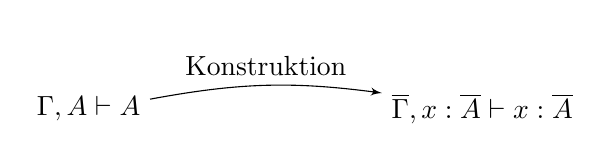
\begin{tikzpicture}[node distance = 5cm]
	\node (a) {$\Gamma,A\PModels A$};
	\uncover<2->{\node[right of = a] (b) {$\trans{\Gamma},x:\trans{A}\lambdaModels x:\trans{A}$};
	\path (a) edge[bend left=9,->,>=latex'] node[above,label] {Konstruktion} (b);}
\end{tikzpicture}
\end{figure}
\end{frame}

\begin{frame}{Beweis}{asd}
\begin{figure}
\centering
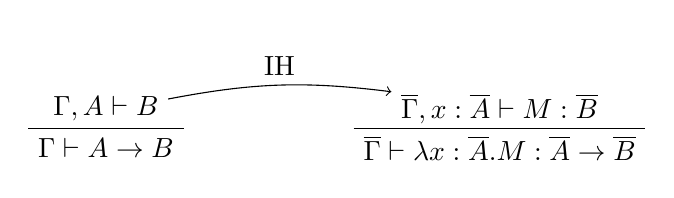
\begin{tikzpicture}[node distance = 0.5cm]
	\node (a1) {$\Gamma\PModels A\to B$};
	\node[above of = a1] (a2) {$\Gamma,A\PModels B$};
	%draw line
	\getwidthofnode{\sright}{a1}
	\draw (a1)+(-\sright/2,+0.25cm) -- +(\sright/2,+0.25cm);
	\uncover<2->{\node[right of = a2,node distance = 5cm] (b2) {$\trans{\Gamma},x:\trans{A}\lambdaModels M:\trans{B}$};
	\path (a2) edge[bend left=9,->] node[above,label] {IH} (b2);
	}
	\uncover<3->{
	\node[right of = a1,node distance = 5cm] (b1) {$\trans{\Gamma}\lambdaModels\lambda x:\trans{A}.M:\trans{A}\to\trans{B}$};
	%draw line
	\getwidthofnode{\sright}{b1}
	\draw (b1)+(-\sright/2,+0.25cm) -- +(\sright/2,+0.25cm);
	}
\end{tikzpicture}
\end{figure}
\end{frame}
%TODO falls zu wenig folien noch ->eli und \forall-Intro

\begin{frame}{Beweis}{asd}
\begin{figure}
\centering
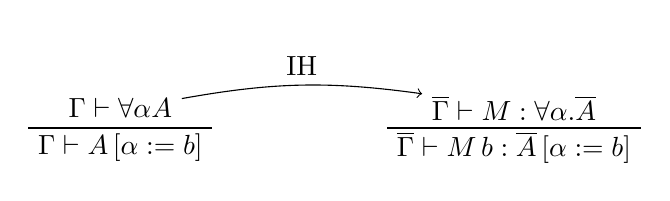
\begin{tikzpicture}[node distance = 0.5cm]
	\node (a1) {$\Gamma\PModels A\left[\alpha:=b\right]$};
	\node[above of = a1] (a2) {$\Gamma\PModels\forall\alpha A$};
	%draw line
	\getwidthofnode{\sright}{a1}
	\draw (a1)+(-\sright/2,+0.25cm) -- +(\sright/2,+0.25cm);
	\uncover<2->{\node[right of = a2,node distance = 5cm] (b2) {$\trans{\Gamma}\lambdaModels M:\forall\alpha.\trans{A}$};
	\path (a2) edge[bend left=9,->] node[above,label] {IH} (b2);
	}
	\uncover<3->{
	\node[right of = a1,node distance = 5cm] (b1) {$\trans{\Gamma}\lambdaModels M\,b:\trans{A}\left[\alpha:=b\right]$};
	%draw line
	\getwidthofnode{\sright}{b1}
	\draw (b1)+(-\sright/2,+0.25cm) -- +(\sright/2,+0.25cm);
	}
\end{tikzpicture}
\end{figure}
\end{frame}

%r�ckrichtung
\begin{frame}{Beweis}{asd}
	\begin{align*}
	\textit{$\Gamma\PModels\false$}&&\Leftarrow&&\textit{Es existiert ein $\lambdaTwo$ Term $M$ sodass  $\trans{\Gamma}\lambdaModels M:\false$}
	\end{align*}
	\uncover<2->{
	\begin{align*}
		\textit{$\trans{\Gamma}\lambdaModels M:\code{P}{s}{t}$}&&\Rightarrow&&\textit{$\Gamma\PModels P(s,t)$}\\
		\textit{$\trans{\Gamma}\lambdaModels M:\false$}&&\Rightarrow&&\textit{$\Gamma\PModels \false$}
	\end{align*}}
	
\end{frame}

\begin{frame}{asd}{asd}
\begin{figure}
	\centering
	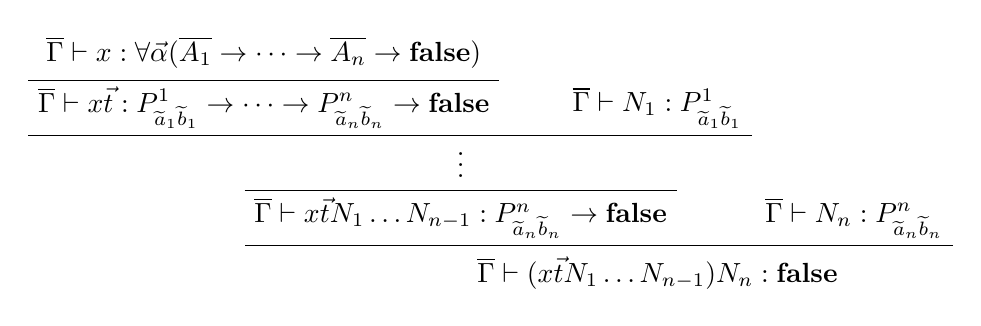
\begin{tikzpicture}[grow=up,level distance=0.7cm,
execute at begin node=$, execute at end node=$,
every node/.style={opacity=1},
every child/.style={edge from parent/.style={opacity=0}}]
\def\dist{0.7cm}
\node(e) {\trans{\Gamma}\lambdaModels (x\vec{t}N_1\dots N_{n-1})N_n:\false} [sibling distance = 5cm]
	child {node(1) {\trans{\Gamma}\lambdaModels N_n:\code{P^n}{\widetilde{a}_n}{\widetilde{b}_n}}}
	child {node(2) {\trans{\Gamma}\lambdaModels x\vec{t}N_1\dots N_{n-1}:\code{P^n}{\widetilde{a}_n}{\widetilde{b}_n}\to\false}
		child {{node[label={[yshift=-0.44cm]above:\vdots}](21) {}}
			child {node(211) {\trans{\Gamma}\lambdaModels N_1:\code{P^1}{\widetilde{a}_1}{\widetilde{b}_1}}}
			child {node(212) {\trans{\Gamma}\lambdaModels x\vec{t}:\code{P^1}{\widetilde{a}_1}{\widetilde{b}_1}\to\dots\to\code{P^n}{\widetilde{a}_n}{\widetilde{b}_n}\to\false}
				child {node(2121) {\trans{\Gamma}\lambdaModels x:\forall\vec{\alpha}(\trans{A_1}\to\dots\to\trans{A_n}\to\false)}}}}};


\def\nodes{,1,2,21,211,212,2121}
\def\identifier{C1:2}
\foreach \x in \nodes{
\ifnodedefined{\x}{
	\coordinate(c\x) at (\x);
	\coordinate(\identifier.\x) at (0,0);
}{}
}
\coordinate(c) at (e);
\def\lvl{3.5mm}

%draw lines for each node with 2 children (add parents with 2 children)
\foreach \x in \nodes{
\ifnodedefined{\identifier.\x1}{
	%calculate with of line
	\getwidthofnode{\sright}{\x1}
	%if there is a right child draw wide line
	\ifnodedefined{\identifier.\x2}{
		\getwidthofnode{\sleft}{\x2}
		%draw line
		\draw[shorten <=-\sright/2, shorten >=-\sleft/2] ([yshift=-\lvl]c\x1) -- ([yshift=-\lvl]c\x2);
	} %else only one child
	{
		\ifnodedefined{\x}
			{\getwidthofnode{\sleft}{\x}}
			{\getwidthofnode{\sleft}{e}}
		%get widht corresponding to the widht of the bigger node
		\pgfmathsetlength{\sright}{max(\sright,\sleft)}
		%draw line
		\draw (c\x)+(-\sright/2,+\lvl) -- +(\sright/2,+\lvl);
	}
}{}
}
\end{tikzpicture}
\end{figure}
\end{frame}
\end{document}